\documentclass[12pt]{article}
\usepackage{fancyhdr}
\usepackage[letterpaper, margin=1in]{geometry}
%\usepackage{indentfirst}
\usepackage{graphicx}
\usepackage{amsmath}
\usepackage{amssymb}
\usepackage{siunitx}
\sisetup{detect-weight=true, detect-family=true} % makes siunitx follow font formatting like bold, italic, etc.
\usepackage{cancel}
\usepackage{isotope}
\usepackage{listings}
\usepackage[dvipsnames,table]{xcolor}
\usepackage{xspace}
\usepackage{booktabs} % makes tables pretty
\usepackage{longtable} % for long tables
\usepackage{multirow} % makes tables pretty
\usepackage{multicol} % makes tables pretty
\usepackage{setspace}
\usepackage{subcaption}
\usepackage{hyperref}
\usepackage{cleveref}
\newcommand{\creflastconjunction}{, and\nobreakspace} % adds oxford comma to cleveref
\usepackage[utf8]{inputenc}
\usepackage{textcomp}
\usepackage{titlesec}
\usepackage{svg}
\usepackage{pdflscape} % makes pages landscape
\usepackage{mathtools}
\usepackage{enumitem}
\usepackage[T1]{fontenc}
\usepackage{tikz}


\doublespacing

% bib if needed
\bibliographystyle{ieeetr}


% fancy header stuff
\usepackage{fancyhdr}
\pagestyle{fancy}

\setlength{\headheight}{28pt}
\lhead{ME 568 / OC 674\\Spring 2022}
\chead{Assignment 4\\}
\rhead{Austin Warren\\Due May 24, 2022}

\begin{document}
	
	\begin{enumerate}
		% Part 1
		\item \textbf{Part 1:} Choose a time when the flow is strongly turbulent and evaluate the following:
		\begin{enumerate}
			\item First perform a Reynolds decomposition by defining the mean and perturbation $u$, $v$, $w$. Because the background state varies in $z$. Discuss any challenges you might have in doing decomposition.\par
			
			I chose the eight time step ($t=\SI{3043.9}{\second}$) because it is far enough along to have turbulence. I also did my analysis only in the second $y$ plane. For the Reynolds decomposition, I decided to average over $x$, such that the mean velocity is only a function of $z$. I did this for the velocity in all three directions. The fluctuating values are then just the difference between the instantaneous velocity and the mean velocity. Normally, the Reynolds decomposition involves a time average, however in this case, the time steps are very far apart and do not provide a sufficient number of data points to provide a good average. The mean as a function of $z$ and $t$ works well because the flow in the $x$-direction is relatively constant at each $z$ value.
			
			
			\begin{figure}[htbp]
				\centering
				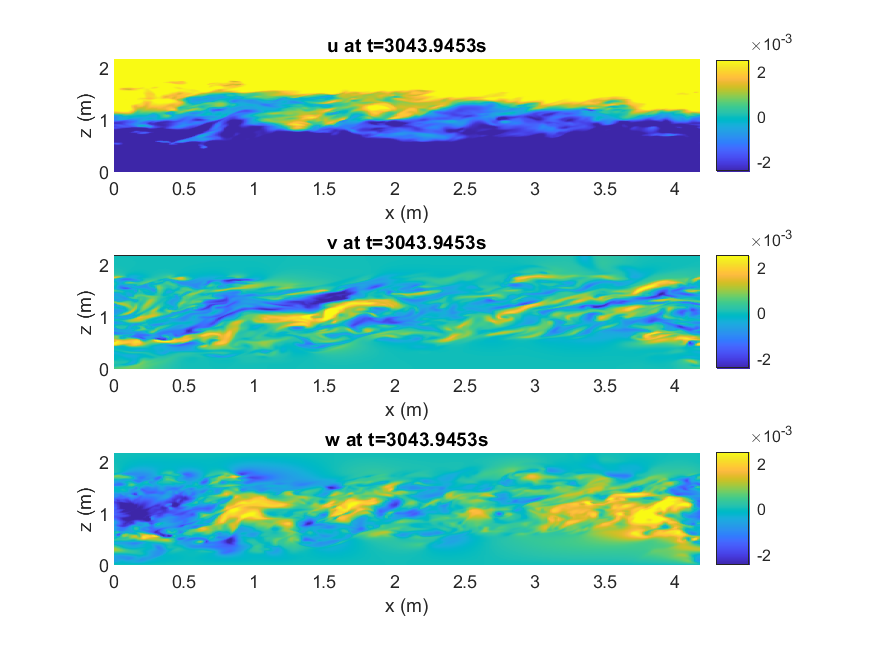
\includegraphics[width=\textwidth]{1-plots/Vel_plot_3043.png}
				\label{fig:Vel 3043}
				\caption{Instantaneous velocity at $t=\SI{3043.9}{\second}$.}
			\end{figure}
		
			\begin{figure}[htbp]
				\centering
				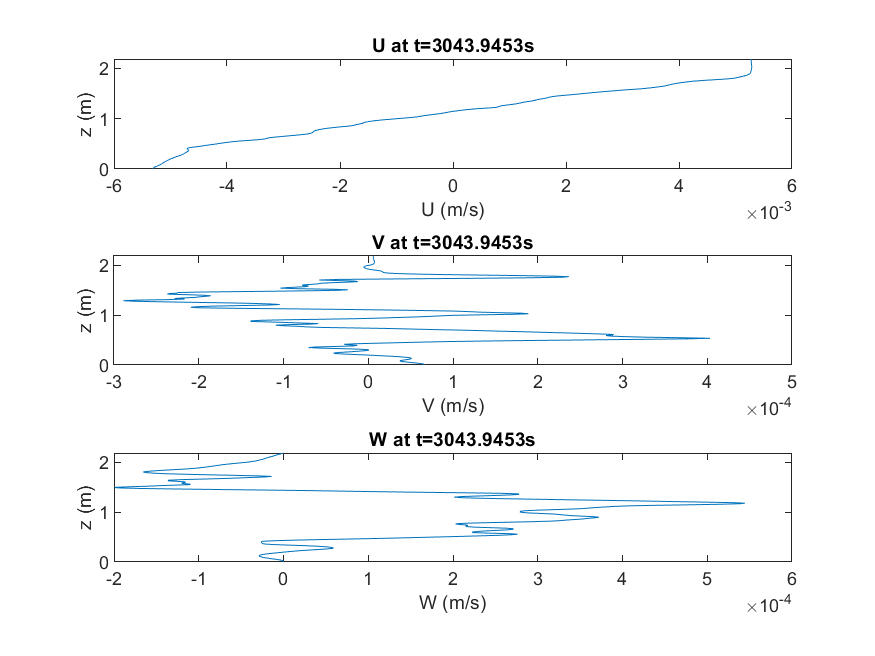
\includegraphics[width=\textwidth]{1-plots/Vel_avg_plot_3043.png}
				\label{fig:Vel avg 3043}
				\caption{Mean velocity at $t=\SI{3043.9}{\second}$.}
			\end{figure}
		
			\begin{figure}[htbp]
				\centering
				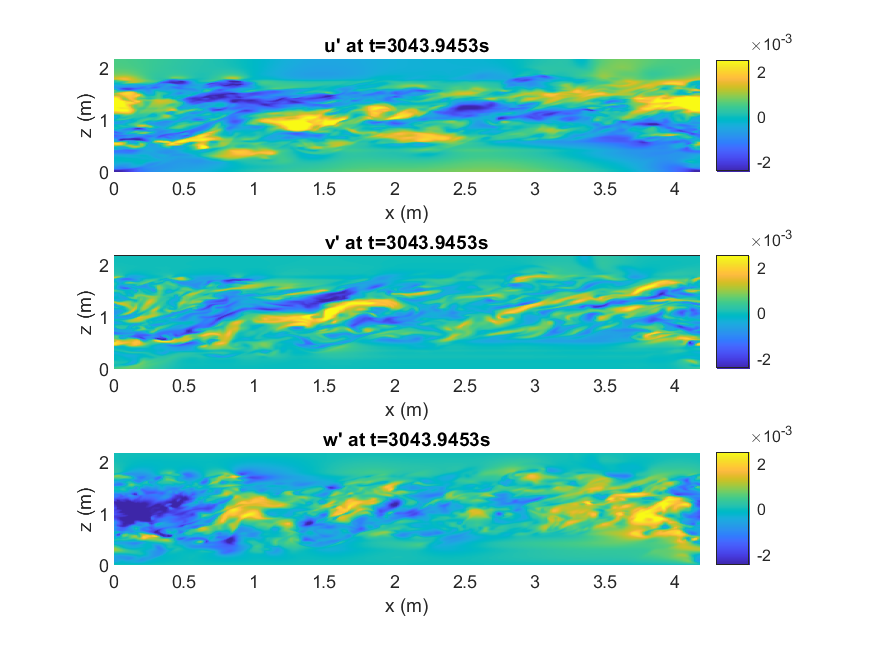
\includegraphics[width=\textwidth]{1-plots/Vel_primes_plot_3043.png}
				\label{fig:Vel prime 3043}
				\caption{Fluctuating velocity at $t=\SI{3043.9}{\second}$.}
			\end{figure}
			
			
			\clearpage
			\item Now that you have decomposed the velocity, compute the individual components of the turbulent kinetic energy and the Reynolds stresses. Discuss any significant features of the patterns or magnitudes.\par
			
			
			
			\begin{figure}[htpb]
				\centering
				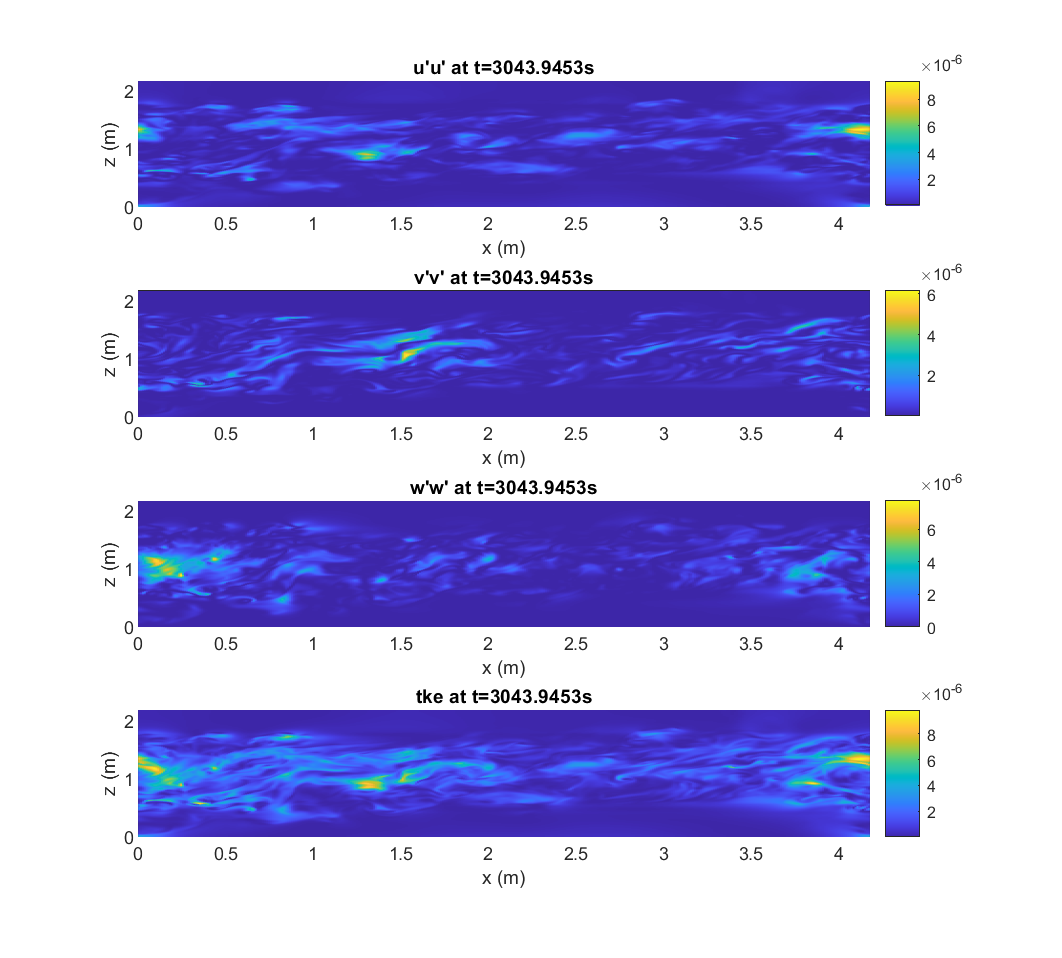
\includegraphics[width=\textwidth]{1-plots/tke_plot_3043.png}
				\label{fig:tke 3043}
				\caption{TKE at $t=\SI{3043.9}{\second}$.}
			\end{figure}
		
			\begin{figure}[htbp]
				\centering
				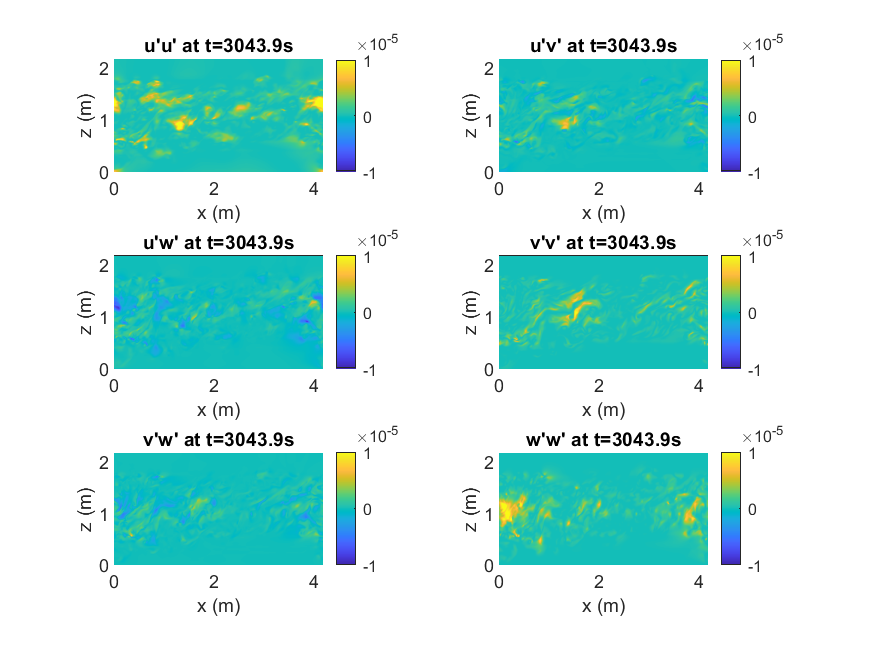
\includegraphics[width=\textwidth]{1-plots/ReynoldsStress_plot_3043.png}
				\label{fig:reynolds 3043}
				\caption{Reynolds stresses at $t=\SI{3043.9}{\second}$.}
			\end{figure}
			
			\clearpage
			\item Perform the same set of calculations for an earlier time in the flow (when the turbulence is perhaps less homogeneous). Discuss any differences in the character of the flow and/or the components of the tke and Reynolds stresses.\par
			
			
			
		\end{enumerate}
	
		\clearpage
		% Part 2
		\item \textbf{Part 2:} For now neglect the buoyancy contributions and
		\begin{enumerate}
			\item compute the shear production and dissipation throughout the domain at some point in time. Determine a horizontal and volume average of each. Does production balance dissipation?\par
			
			
			\item Once you are satisfied that you can compute production and dissipation (i.e., (a) above), compute the average of each for every timestep and plot a time series. Does production equal dissipation on average? Write a paragraph describing the production and dissipation evolution.
		\end{enumerate}
	
	
		\clearpage
		% Part 3
		\item \textbf{Part 3:} Now consider the buoyancy production term.
		\begin{enumerate}
			\item Compute time-integrals of the spatially-integrated buoyancy production $J_b$ and compare this to shear production and dissipation. Does this help to account for any mismatches above? If there are mismatches and you can't close the energy budget, explain what might be the problem.
			
			
			\item  Now try to compare these to the integrated TKE production and the total change in potential energy due to mixing within the simulation domain. Can you close an energy budget, and if not, what might be the problem? What is the mixing efficiency? Which measure of the total mixing is most robust?
		
		\end{enumerate}
		
	\end{enumerate}
		
	
	
	
	
	
	
	
	
	
\end{document}